\begin{slide}{Execution Model}
\begin{center}
  \only<2>{
  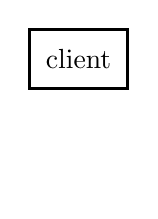
\begin{tikzpicture}
  % Client
  \draw [very thick] (0, 0) rectangle ++(1.25, 0.75) node [midway] {client};

  % Spacing node
  \draw (0, -1.3);
  \end{tikzpicture}
  }
  \only<3>{
    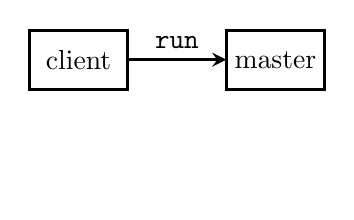
\begin{tikzpicture}
  % Client
  \draw [very thick] (0, 0) rectangle ++(1.25, 0.75) node [midway] {client};

  % Master
  \draw [very thick] (2.5, 0) rectangle ++(1.25, 0.75) node [midway] {master};
  \draw [very thick, -stealth] (1.25, 0.375) -- (2.5, 0.375) node [midway,
    above] {\texttt{run}};

  % Spacing node
  \draw (0, -1.3);
  \end{tikzpicture}
  }
  \only<4>{
    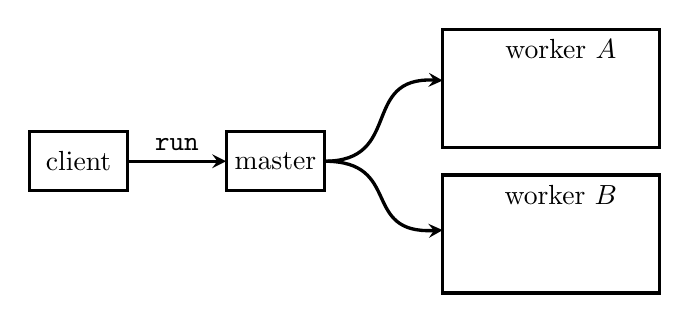
\begin{tikzpicture}
  % Client
  \draw [very thick] (0, 0) rectangle ++(1.25, 0.75) node [midway] {client};

  % Master
  \draw [very thick] (2.5, 0) rectangle ++(1.25, 0.75) node [midway] {master};
  \draw [very thick, -stealth] (1.25, 0.375) -- (2.5, 0.375) node [midway,
    above] {\texttt{run}};

  % Worker 1
  \draw [very thick] (5.25, 0.55) rectangle ++(2.75, 1.5);
  \draw (6.75, 1.8) node {worker $A$};

  % Worker 2
  \draw [very thick] (5.25, -1.3) rectangle ++(2.75, 1.5);
  \draw (6.75, -0.05) node {worker $B$};

  % Edges
  \draw [very thick, -stealth]
        (3.75, 0.375) .. controls +(1, 0) and (4.2, 1.45) .. (5.25, 1.4);
  \draw [very thick, -stealth]
        (3.75, 0.375) .. controls +(1, 0) and (4.2, -0.55) .. (5.25, -0.5);
  \end{tikzpicture}
  }
  \only<5>{
    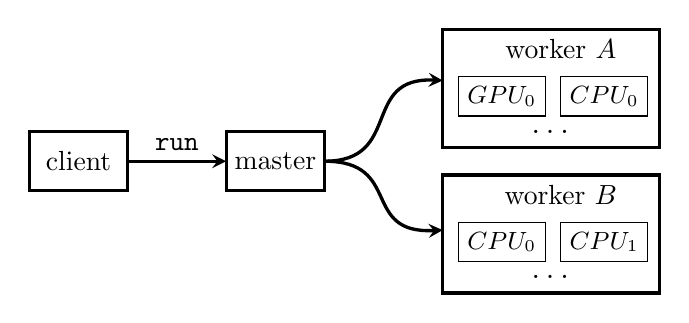
\begin{tikzpicture}
  % Client
  \draw [very thick] (0, 0) rectangle ++(1.25, 0.75) node [midway] {client};

  % Master
  \draw [very thick] (2.5, 0) rectangle ++(1.25, 0.75) node [midway] {master};
  \draw [very thick, -stealth] (1.25, 0.375) -- (2.5, 0.375) node [midway,
    above] {\texttt{run}};

  % Worker 1
  \draw [very thick] (5.25, 0.55) rectangle ++(2.75, 1.5);
  \draw (6.75, 1.8) node {worker $A$};
  \draw (5.45, 0.95) rectangle ++(1.1, 0.5) node [midway] {\small$GPU_0$};
  \draw (6.75, 0.95) rectangle ++(1.1, 0.5) node [midway] {\small$CPU_0$};
  \draw (6.65, 0.75) node {\large\dots};


  % Worker 2
  \draw [very thick] (5.25, -1.3) rectangle ++(2.75, 1.5);
  \draw (6.75, -0.05) node {worker $B$};
  \draw (5.45, -0.9) rectangle ++(1.1, 0.5) node [midway] {\small$CPU_0$};
  \draw (6.75, -0.9) rectangle ++(1.1, 0.5) node [midway] {\small$CPU_1$};
  \draw (6.65, -1.1) node {\large\dots};

  % Edges
  \draw [very thick, -stealth]
        (3.75, 0.375) .. controls +(1, 0) and (4.2, 1.45) .. (5.25, 1.4);
  \draw [very thick, -stealth]
        (3.75, 0.375) .. controls +(1, 0) and (4.2, -0.55) .. (5.25, -0.5);
  \end{tikzpicture}
  }
  \only<6>{
    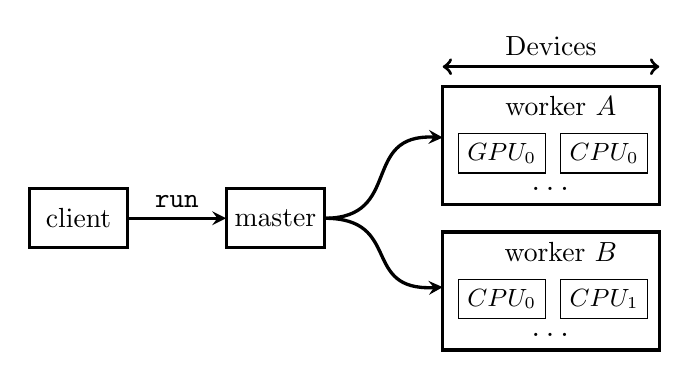
\begin{tikzpicture}
  % Client
  \draw [very thick] (0, 0) rectangle ++(1.25, 0.75) node [midway] {client};

  % Master
  \draw [very thick] (2.5, 0) rectangle ++(1.25, 0.75) node [midway] {master};
  \draw [very thick, -stealth] (1.25, 0.375) -- (2.5, 0.375) node [midway,
    above] {\texttt{run}};

  % Worker 1
  \draw [very thick] (5.25, 0.55) rectangle ++(2.75, 1.5);
  \draw (6.75, 1.8) node {worker $A$};
  \draw (5.45, 0.95) rectangle ++(1.1, 0.5) node [midway] {\small$GPU_0$};
  \draw (6.75, 0.95) rectangle ++(1.1, 0.5) node [midway] {\small$CPU_0$};
  \draw (6.65, 0.75) node {\large\dots};


  % Worker 2
  \draw [very thick] (5.25, -1.3) rectangle ++(2.75, 1.5);
  \draw (6.75, -0.05) node {worker $B$};
  \draw (5.45, -0.9) rectangle ++(1.1, 0.5) node [midway] {\small$CPU_0$};
  \draw (6.75, -0.9) rectangle ++(1.1, 0.5) node [midway] {\small$CPU_1$};
  \draw (6.65, -1.1) node {\large\dots};

  % Edges
  \draw [very thick, -stealth]
        (3.75, 0.375) .. controls +(1, 0) and (4.2, 1.45) .. (5.25, 1.4);
  \draw [very thick, -stealth]
        (3.75, 0.375) .. controls +(1, 0) and (4.2, -0.55) .. (5.25, -0.5);

  % Device Scalability
  \draw [very thick, <->] (5.25, 2.3) -- ++(2.75, 0)
        node [midway, above] {Devices};
  \end{tikzpicture}
  }
  \only<7>{
    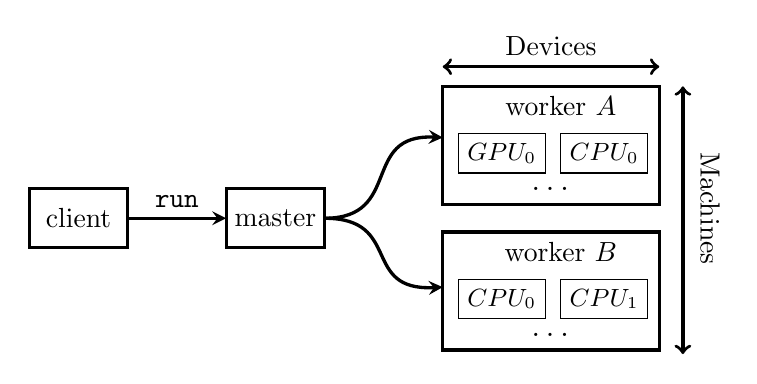
\begin{tikzpicture}
  % Client
  \draw [very thick] (0, 0) rectangle ++(1.25, 0.75) node [midway] {client};

  % Master
  \draw [very thick] (2.5, 0) rectangle ++(1.25, 0.75) node [midway] {master};
  \draw [very thick, -stealth] (1.25, 0.375) -- (2.5, 0.375) node [midway,
    above] {\texttt{run}};

  % Worker 1
  \draw [very thick] (5.25, 0.55) rectangle ++(2.75, 1.5);
  \draw (6.75, 1.8) node {worker $A$};
  \draw (5.45, 0.95) rectangle ++(1.1, 0.5) node [midway] {\small$GPU_0$};
  \draw (6.75, 0.95) rectangle ++(1.1, 0.5) node [midway] {\small$CPU_0$};
  \draw (6.65, 0.75) node {\large\dots};


  % Worker 2
  \draw [very thick] (5.25, -1.3) rectangle ++(2.75, 1.5);
  \draw (6.75, -0.05) node {worker $B$};
  \draw (5.45, -0.9) rectangle ++(1.1, 0.5) node [midway] {\small$CPU_0$};
  \draw (6.75, -0.9) rectangle ++(1.1, 0.5) node [midway] {\small$CPU_1$};
  \draw (6.65, -1.1) node {\large\dots};

  % Edges
  \draw [very thick, -stealth]
        (3.75, 0.375) .. controls +(1, 0) and (4.2, 1.45) .. (5.25, 1.4);
  \draw [very thick, -stealth]
        (3.75, 0.375) .. controls +(1, 0) and (4.2, -0.55) .. (5.25, -0.5);

  % Device Scalability
  \draw [very thick, <->] (5.25, 2.3) -- ++(2.75, 0)
        node [midway, above] {Devices};

  % Machine Scalability
  \draw [very thick, <->] (8.3, -1.35) -- ++(0, 3.4);
  \draw (8.4, 0.5) node [rotate=270, above] {Machines};
  \end{tikzpicture}
  }

  \onslide<2->{
    \textbf{Actors}
    \\ \vspace{0.3cm}
    \inlineitem{1}{Client}
  }
  \onslide<3->{\inlineitem{2}{Master}}
  \onslide<4->{\inlineitem{3}{Workers}}
  \onslide<5->{\inlineitem{4}{Devices}}
\end{center}
\end{slide}

%%% Local Variables:
%%% mode: latex
%%% TeX-master: "../presentation.tex"
%%% End: